
\begin{frame}
\frametitle{Expansion or Truncation?}
\begin{itemize}
\item Many sources per FGT box $-$ Expansion
\newline
\item Few sources per FGT box $-$ Truncation
\newline
\item Non-uniform distributions $-$ Hybrid
\end{itemize}
\end{frame}


\begin{frame}
\frametitle{Octree based FGT}
\framesubtitle{Tree construction}
\begin{columns}[T]
\begin{column}{0.4\textwidth}
\begin{itemize}
\item Max. of $m$ points per leaf
\only<2->{
\item Higher point density $\Rightarrow$ finer leaves
}
\only<3>{
\item Large leaves $\Rightarrow$ Truncation ({\color{blue}{Direct}})
\item Small leaves $\Rightarrow$ Expansion ({\color{green!65!black}{Expand}})
}
\end{itemize}
\end{column}
\begin{column}{0.6\textwidth}
\only<1> {

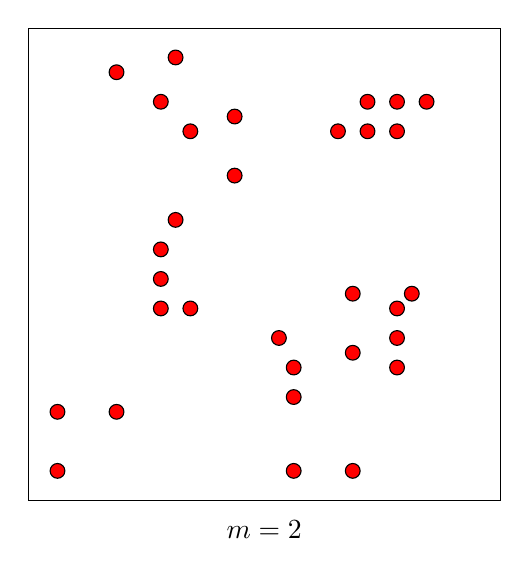
\begin{tikzpicture}[scale=0.75]
	    	% domain boundary 
	  			  		
	  		\draw[black, very thin] (0,0) rectangle (8,8);
	  		  		
	  		
	  			%% points ...	  		
	  		\draw[fill=red] (2.25,3.75) circle (0.125);
	  		\draw[fill=red] (2.25,3.25) circle (0.125);
	  		\draw[fill=red] (1.5,1.5) circle (0.125);
	  		\draw[fill=red] (0.5,1.5) circle (0.125);	
	  		
	  		\draw[fill=red] (4.5,0.5) circle (0.125);
	  		\draw[fill=red] (5.5,0.5) circle (0.125);
	  		\draw[fill=red] (5.5,2.5) circle (0.125);
	  		\draw[fill=red] (5.5,3.5) circle (0.125);	  		
	  		\draw[fill=red] (6.5,3.5) circle (0.125);
	  		
	  		
	  		\draw[fill=red] (3.5,5.5) circle (0.125);
	  		\draw[fill=red] (3.5,6.5) circle (0.125);
	  		\draw[fill=red] (2.5,7.5) circle (0.125);
	  		
	  		\draw[fill=red] (6.25,6.25) circle (0.125);
	  		\draw[fill=red] (6.75,6.75) circle (0.125);
	  		\draw[fill=red] (5.25,6.25) circle (0.125);
	  		\draw[fill=red] (5.75,6.75) circle (0.125);

        \draw[fill=red] (0.5, 0.5) circle (0.125);
	  		\draw[fill=red] (1.5, 7.25) circle (0.125);	  		
	  		\draw[fill=red] (2.25, 4.25) circle (0.125);
	  		\draw[fill=red] (2.5,4.75) circle (0.125);
	  		\draw[fill=red] (2.75, 3.25) circle (0.125);
	  		\draw[fill=red] (4.5, 1.75) circle (0.125);
	  		\draw[fill=red] (2.75, 6.25) circle (0.125);
	  		\draw[fill=red] (4.25, 2.75) circle (0.125);
	  		\draw[fill=red] (6.25,2.75) circle (0.125);
	  		\draw[fill=red] (6.25,2.25) circle (0.125);
	  		\draw[fill=red] (6.25,3.25) circle (0.125);
	  		\draw[fill=red] (5.75,6.25) circle (0.125);
	  		\draw[fill=red] (6.25,6.75) circle (0.125);
	  		\draw[fill=red] (2.25,6.75) circle (0.125);
	  		\draw[fill=red] (4.5,2.25) circle (0.125);
	  		
				\draw (4,-0.5) node {$m = 2$};
	  		
   	\end{tikzpicture}  
   	
   	
}
\only<2> {
\input{pointsDemoOut}
}
\only<3> {

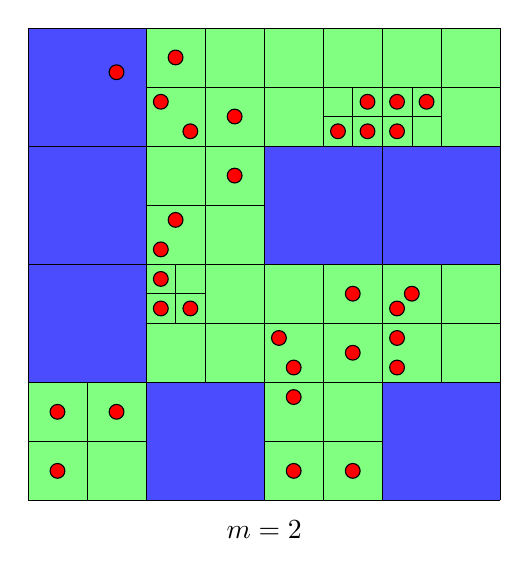
\begin{tikzpicture}[scale=0.75]

				\fill[blue!70] (2,0) rectangle (4,2);
				\fill[blue!70] (0,2) rectangle (2,8);
				\fill[blue!70] (4,4) rectangle (8,6);
				\fill[blue!70] (6,0) rectangle (8,2);
				
 				\fill[green!50] (0,0) rectangle (2,2); 				
 				\fill[green!50] (2,2) rectangle (4,8);
 				\fill[green!50] (4,0) rectangle (6,4);
 				\fill[green!50] (6,2) rectangle (8,4);
 				\fill[green!50] (4,6) rectangle (8,8);
	  		
	  		%% points ...	  		
	  		\draw[fill=red] (2.25,3.75) circle (0.125);
	  		\draw[fill=red] (2.25,3.25) circle (0.125);
	  		\draw[fill=red] (1.5,1.5) circle (0.125);
	  		\draw[fill=red] (0.5,1.5) circle (0.125);	
	  		
	  		\draw[fill=red] (4.5,0.5) circle (0.125);
	  		\draw[fill=red] (5.5,0.5) circle (0.125);
	  		\draw[fill=red] (5.5,2.5) circle (0.125);
	  		\draw[fill=red] (5.5,3.5) circle (0.125);	  		
	  		\draw[fill=red] (6.5,3.5) circle (0.125);
	  		
	  		
	  		\draw[fill=red] (3.5,5.5) circle (0.125);
	  		\draw[fill=red] (3.5,6.5) circle (0.125);
	  		\draw[fill=red] (2.5,7.5) circle (0.125);
	  		
	  		\draw[fill=red] (6.25,6.25) circle (0.125);
	  		\draw[fill=red] (6.75,6.75) circle (0.125);
	  		\draw[fill=red] (5.25,6.25) circle (0.125);
	  		\draw[fill=red] (5.75,6.75) circle (0.125);

        \draw[fill=red] (0.5, 0.5) circle (0.125);
	  		\draw[fill=red] (1.5, 7.25) circle (0.125);	  		
	  		\draw[fill=red] (2.25, 4.25) circle (0.125);
	  		\draw[fill=red] (2.5,4.75) circle (0.125);
	  		\draw[fill=red] (2.75, 3.25) circle (0.125);
	  		\draw[fill=red] (4.5, 1.75) circle (0.125);
	  		\draw[fill=red] (2.75, 6.25) circle (0.125);
	  		\draw[fill=red] (4.25, 2.75) circle (0.125);
	  		\draw[fill=red] (6.25,2.75) circle (0.125);
	  		\draw[fill=red] (6.25,2.25) circle (0.125);
	  		\draw[fill=red] (6.25,3.25) circle (0.125);
	  		\draw[fill=red] (5.75,6.25) circle (0.125);
	  		\draw[fill=red] (6.25,6.75) circle (0.125);
	  		\draw[fill=red] (2.25,6.75) circle (0.125);
	  		\draw[fill=red] (4.5,2.25) circle (0.125);
	  		  		
	  		
				\draw (4,-0.5) node {$m = 2$};

	    	% domain boundary 
	  		\draw[black, very thin, step=2] (0,0) grid (8,8);
	  		\draw[black, very thin, step=1] (0,0) grid (2,2);
	  		\draw[black, very thin, step=1] (2,2) grid (4,4);
	  		\draw[black, very thin, step=1] (4,0) grid (6,4);
	  		\draw[black, very thin, step=1] (6,2) grid (8,4);
	  		\draw[black, very thin, step=1] (2,4) grid (4,8);
	  		\draw[black, very thin, step=1] (4,6) grid (8,8);
	  		\draw[black, very thin, step=0.5] (2,3) grid (3,4);
	  		\draw[black, very thin, step=0.5] (5,6) grid (7,7);

	  		
   	\end{tikzpicture}  
}
\end{column}
\end{columns}
\end{frame}


\begin{frame}
\frametitle{Octree based FGT}
\framesubtitle{Flow of Information}
\begin{itemize}
\item Source $-$ $y$
\item Target $-$ $x$
\item {\color{blue}{Direct}} tree $-$ {\color{blue}{$T_d$}}
\item {\color{green!65!black}{Expand}} tree $-$ {\color{green!65!black}{$T_e$}}
\end{itemize}

\vspace{-0.25cm}

\only<1> {
\bean
y & x &  \\
{\color{green!65!black}{T_e}} & {\color{green!65!black}{T_e}} & {\color{green!65!black}{y}} \xrightarrow[]{\textbf{S2W}} \{ w_k\} \xrightarrow[]{\textbf{W2L}} \{ v_k \}\xrightarrow[]{\textbf{L2T}} {\color{green!65!black}{x}}  \\
{\color{green!65!black}{T_e}} & {\color{blue}{T_d}} & {\color{green!65!black}{y}} \xrightarrow[]{\textbf{S2W}} \{ w_k\} \xrightarrow[]{\textbf{W2D}} {\color{blue}{x}}  \\
{\color{blue}{T_d}} & {\color{green!65!black}{T_e}} & {\color{blue}{y}} \xrightarrow[]{\textbf{D2L}} \{ v_k \}\xrightarrow[]{\textbf{L2T}} {\color{green!65!black}{x}}  \\
{\color{blue}{T_d}} & {\color{blue}{T_d}} & {\color{blue}{y}} \xrightarrow[]{\textbf{D2D}} {\color{blue}{x}}  \\
\eean
}

\only<2> {
\bean
y & x &  \\
{\color{green!65!black}{T_e}} & {\color{green!65!black}{T_e}} & {\color{green!65!black}{y}} \xrightarrow[]{\textbf{S2W}} \{ w_k\} \xrightarrow[]{\textbf{W2L}} \{ v_k \}\xrightarrow[]{\textbf{L2T}} {\color{green!65!black}{x}}  \\
{\color{green!65!black}{T_e}} & {\color{blue}{T_d}} & {\color{green!65!black}{y}} \xrightarrow[]{\textbf{S2W}} \{ w_k\} \xrightarrow[]{\color{red}{\textbf{W2D}}} {\color{blue}{x}} \, \color{red}{\left[ F(x) \, +=\, \sum_{|k| \leq p} \hat{G}(k)  w_k e^{i \lambda k \cdot (x - c^B)} \right]} \\
{\color{blue}{T_d}} & {\color{green!65!black}{T_e}} & {\color{blue}{y}} \xrightarrow[]{\textbf{D2L}} \{ v_k \}\xrightarrow[]{\textbf{L2T}} {\color{green!65!black}{x}}  \\
{\color{blue}{T_d}} & {\color{blue}{T_d}} & {\color{blue}{y}} \xrightarrow[]{\textbf{D2D}} {\color{blue}{x}}  \\
\eean
}

\only<3> {
\bean
y & x &  \\
{\color{green!65!black}{T_e}} & {\color{green!65!black}{T_e}} & {\color{green!65!black}{y}} \xrightarrow[]{\textbf{S2W}} \{ w_k\} \xrightarrow[]{\textbf{W2L}} \{ v_k \}\xrightarrow[]{\textbf{L2T}} {\color{green!65!black}{x}}  \\
{\color{green!65!black}{T_e}} & {\color{blue}{T_d}} & {\color{green!65!black}{y}} \xrightarrow[]{\textbf{S2W}} \{ w_k\} \xrightarrow[]{\color{red}{\textbf{W2D}}} {\color{blue}{x}} \, \color{red}{\left[ F(x) \, +=\, \sum_{|k| \leq p} \hat{G}(k)  w_k e^{i \lambda k \cdot (x - c^B)} \right]} \\
{\color{blue}{T_d}} & {\color{green!65!black}{T_e}} & {\color{blue}{y}} \xrightarrow[]{\color{red}{\textbf{D2L}}} \{ v_k \}\xrightarrow[]{\textbf{L2T}} {\color{green!65!black}{x}} \, \color{red}{\left[ v_k  \,+=\, \, f(y) e^{i \lambda k \cdot (c^D - y)} \right]} \\
{\color{blue}{T_d}} & {\color{blue}{T_d}} & {\color{blue}{y}} \xrightarrow[]{\textbf{D2D}} {\color{blue}{x}}  \\
\eean
}

\only<4> {
\bean
y & x &  \\
{\color{green!65!black}{T_e}} & {\color{green!65!black}{T_e}} & {\color{green!65!black}{y}} \xrightarrow[]{\textbf{S2W}} \{ w_k\} \xrightarrow[]{\textbf{W2L}} \{ v_k \}\xrightarrow[]{\textbf{L2T}} {\color{green!65!black}{x}}  \\
{\color{green!65!black}{T_e}} & {\color{blue}{T_d}} & {\color{green!65!black}{y}} \xrightarrow[]{\textbf{S2W}} \{ w_k\} \xrightarrow[]{\color{red}{\textbf{W2D}}} {\color{blue}{x}} \, \color{red}{\left[ F(x) \, +=\, \sum_{|k| \leq p} \hat{G}(k)  w_k e^{i \lambda k \cdot (x - c^B)} \right]} \\
{\color{blue}{T_d}} & {\color{green!65!black}{T_e}} & {\color{blue}{y}} \xrightarrow[]{\color{red}{\textbf{D2L}}} \{ v_k \}\xrightarrow[]{\textbf{L2T}} {\color{green!65!black}{x}} \, \color{red}{\left[ v_k  \,+=\, \, f(y) e^{i \lambda k \cdot (c^D - y)} \right]} \\
{\color{blue}{T_d}} & {\color{blue}{T_d}} & {\color{blue}{y}} \xrightarrow[]{\color{red}{\textbf{D2D}}} {\color{blue}{x}} \, \color{red}{\left[ F(x) \,+=\, G_\delta(\norm{x - y}) f(y) \right]}  \\
\eean
}

\end{frame}

\begin{frame}
\frametitle{Octree based FGT}
\framesubtitle{Data Partition}
\begin{columns}[T]
\begin{column}{0.6\textwidth}
\begin{itemize}
\item Distributed regular grid of FGT boxes
\begin{itemize}
\item Each box owned by an unique CPU
\item Each CPU owns a sub-grid of boxes
\item PETSc package
\end{itemize}
\item Distributed octree
\begin{itemize}
\item Each leaf owned by an unique CPU
\item Sorted in Morton (space-filling) order
\item {\color{red!40!black}{Direct}} and Expand trees partitioned independently
\item Dendro package 
\end{itemize}
\item Distributed points $-$ mapped to enclosing leaf
\end{itemize}
\end{column}
\begin{column}{0.4\textwidth}

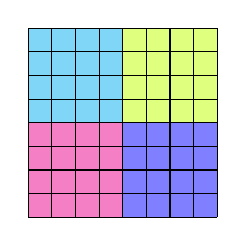
\begin{tikzpicture}[scale=0.6]

    \fill[magenta, opacity=0.5] (0,0) rectangle +(2,2);    
    \fill[blue, opacity=0.5] (2,0) rectangle +(2,2);
    \fill[cyan, opacity=0.5] (0,2) rectangle +(2,2);
    \fill[lime, opacity=0.5] (2,2) rectangle +(2,2);
    
    \draw[step = 0.5] (0,0) grid (4,4);
	  		
\end{tikzpicture}  
\newline

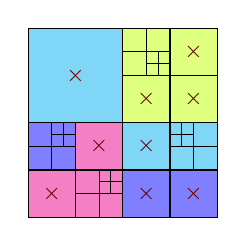
\begin{tikzpicture}[scale=0.6]

  \draw[fill = magenta, fill opacity=0.5] (0,0) rectangle +(1,1);
  \draw (0.5, 0.5) node {\color{red!40!black}{\footnotesize{$\times$}}};
  \draw[fill = magenta, fill opacity=0.5] (1,0) rectangle +(0.5, 0.5);  
  \draw[fill = magenta, fill opacity=0.5] (1.5,0) rectangle +(0.5,0.5);  
  \draw[fill = magenta, fill opacity=0.5] (1,0.5) rectangle +(0.5,0.5);
  \draw[fill = magenta, fill opacity=0.5] (1.5,0.5) rectangle +(0.25,0.25);  
  \draw[fill = magenta, fill opacity=0.5] (1.75,0.5) rectangle +(0.25,0.25);
  \draw[fill = magenta, fill opacity=0.5] (1.5,0.75) rectangle +(0.25,0.25);
  \draw[fill = magenta, fill opacity=0.5] (1.75,0.75) rectangle +(0.25,0.25);
  
  \draw[fill = blue, fill opacity=0.5] (0,1) rectangle +(0.5,0.5);  
  \draw[fill = blue, fill opacity=0.5] (0.5,1) rectangle +(0.5,0.5);
  \draw[fill = blue, fill opacity=0.5] (0,1.5) rectangle +(0.5,0.5);
  \draw[fill = blue, fill opacity=0.5] (0.5,1.5) rectangle +(0.25,0.25);
  \draw[fill = blue, fill opacity=0.5] (0.75,1.5) rectangle +(0.25,0.25);
  \draw[fill = blue, fill opacity=0.5] (0.5,1.75) rectangle +(0.25,0.25);
  \draw[fill = blue, fill opacity=0.5] (0.75,1.75) rectangle +(0.25,0.25);
  
  \draw[fill = magenta, fill opacity=0.5] (1,1) rectangle +(1,1);  
  \draw (1.5, 1.5) node {\color{red!40!black}{\footnotesize{$\times$}}};
  
  \draw[fill = blue, fill opacity=0.5] (2,0) rectangle +(1,1);
  \draw (2.5, 0.5) node {\color{red!40!black}{\footnotesize{$\times$}}};
  \draw[fill = blue, fill opacity=0.5] (3,0) rectangle +(1,1);
  \draw (3.5, 0.5) node {\color{red!40!black}{\footnotesize{$\times$}}};
  
  \draw[fill = cyan, fill opacity=0.5] (2,1) rectangle +(1,1);
  \draw (2.5, 1.5) node {\color{red!40!black}{\footnotesize{$\times$}}};
  \draw[fill = cyan, fill opacity=0.5] (3,1) rectangle +(0.5,0.5);
  \draw[fill = cyan, fill opacity=0.5] (3.5,1) rectangle +(0.5,0.5);
  \draw[fill = cyan, fill opacity=0.5] (3,1.5) rectangle +(0.25,0.25);
  \draw[fill = cyan, fill opacity=0.5] (3.25,1.5) rectangle +(0.25,0.25);
  \draw[fill = cyan, fill opacity=0.5] (3,1.75) rectangle +(0.25,0.25);
  \draw[fill = cyan, fill opacity=0.5] (3.25,1.75) rectangle +(0.25,0.25);
  \draw[fill = cyan, fill opacity=0.5] (3.5,1.5) rectangle +(0.5,0.5);    
  \draw[fill = cyan, fill opacity=0.5] (0,2) rectangle +(2,2);
  \draw (1, 3) node {\color{red!40!black}{\footnotesize{$\times$}}};
  
  \draw[fill = lime, fill opacity=0.5] (2,2) rectangle +(1,1);
  \draw (2.5, 2.5) node {\color{red!40!black}{\footnotesize{$\times$}}};
  \draw[fill = lime, fill opacity=0.5] (3,2) rectangle +(1,1);
  \draw (3.5, 2.5) node {\color{red!40!black}{\footnotesize{$\times$}}};
  \draw[fill = lime, fill opacity=0.5] (2,3) rectangle +(0.5,0.5);
  \draw[fill = lime, fill opacity=0.5] (2.5,3) rectangle +(0.25,0.25);
  \draw[fill = lime, fill opacity=0.5] (2.75,3) rectangle +(0.25,0.25);
  \draw[fill = lime, fill opacity=0.5] (2.5,3.25) rectangle +(0.25,0.25);
  \draw[fill = lime, fill opacity=0.5] (2.75,3.25) rectangle +(0.25,0.25);
  \draw[fill = lime, fill opacity=0.5] (2,3.5) rectangle +(0.5,0.5);
  \draw[fill = lime, fill opacity=0.5] (2.5,3.5) rectangle +(0.5,0.5);
  \draw[fill = lime, fill opacity=0.5] (3,3) rectangle +(1,1);
  \draw (3.5, 3.5) node {\color{red!40!black}{\footnotesize{$\times$}}};
	  		
\end{tikzpicture}  
\end{column}
\end{columns}
\end{frame}

\begin{frame}
\frametitle{Octree based FGT}
\framesubtitle{Parallel Algorithm}
\begin{enumerate}
\item<1-> S2W 
\only<1>{
\begin{enumerate}[(A)]
\item CPUs containing {\color{green!65!black}{Expand}} sources compute plane wave expansions
\item Send expansions to owners of respective FGT boxes
\item Add received values to existing plane wave expansions
\end{enumerate}
}
\item<2-> W2D
\only<2>{
\begin{enumerate}[(A)]
\item CPUs containing {\color{blue}{Direct}} targets form a list of {\em{relevant}} FGT boxes
\item Request plane wave expansions for these boxes from their owners
\item Update transform at {\color{blue}{Direct}} targets using received values
\end{enumerate}
}
\item<3-> D2D
\only<3>{
\begin{enumerate}[(A)]
\item Send {\color{blue}{Direct}} sources to CPUs containing {\em{relevant}} {\color{blue}{Direct}} leaves
\item Update transform at {\color{blue}{Direct}} targets using received values
\end{enumerate}
}
\item<4-> W2L
\only<4>{
\begin{enumerate}[(A)]
\item Communicate plane wave expansions of {\em{ghost}} FGT boxes
\item Execute translation/sweeping algorithm
\end{enumerate}
}
\item<5-> D2L
\only<5>{
\begin{enumerate}[(A)]
\item CPUs containing {\color{blue}{Direct}} sources compute their contributions to {\em{relevant}} FGT boxes
\item Send these contributions to owners of respective FGT boxes
\item Update local expansions using received values 
\end{enumerate}
}
\item<6> L2T
\only<6>{
\begin{enumerate}[(A)]
\item Send local expansions to CPUs containing {\em{relevant}} {\color{green!65!black}{Expand}} targets
\item Compute transform at {\color{green!65!black}{Expand}} targets using received values
\end{enumerate}
}
\end{enumerate}
\end{frame}
